\documentclass[french,10pt]{report}
\input preambule_2014

\begin{document}

Arbres de probabilités :

%---- On définit ci-dessous les différents styles en fonction du niveau dans l'arbre de proba :
\tikzstyle{level 1}=[level distance=2cm,sibling distance=-3cm]
\tikzstyle{level 2}=[level distance=2.5cm,sibling distance=-1.5cm]
\tikzstyle{level 3}=[level distance=2.5cm,sibling distance=-1.5cm]

%---- sibling distance négative => les noeuds sont compilés de haut en bas

\begin{tikzpicture}
[grow=right] % dessine l'arbre de gauche à droite. Les options left, up et down sont également disponibles.
    \node{$\Omega$}
%----------------------------------------------------------------------------------------------------------------------
%----------------------------------------------------------------------------------------------------------------------
        child {node(A1) {A}
%----------------------------------------------------------------------------------------------------------------------
                child {node (B1) {B} % le nom du noeud entre parenthèses permet de réutiliser ce noeud ultérieurement (cf tout en bas)
                         edge from parent node[above] {$P_A(B)$}
                        }
%----------------------------------------------------------------------------------------------------------------------
                child {node(B2) {$\overline{B}$}
                         edge from parent node[below] {$P_A(\overline{B})$}
                        }
%----------------------------------------------------------------------------------------------------------------------
           edge from parent node[above] {$P(A)$}
        }
%----------------------------------------------------------------------------------------------------------------------
%----------------------------------------------------------------------------------------------------------------------
        child {node {$\overline{A}$}
%----------------------------------------------------------------------------------------------------------------------
                child {node(B3) {B}
                        edge from parent node[above] {$P_{\overline{A}}(B)$}
                        }
%----------------------------------------------------------------------------------------------------------------------
                child {node(B4) {$\overline{B}$}
                         edge from parent node[below] {$P_{\overline{A}}(\overline{B})$}
                        }
%----------------------------------------------------------------------------------------------------------------------
            edge from parent node[below] {$P(\overline{A})$}
        }
;
% Utilisation d'un noeud déjà défini
% ligne du haut : tout est défini en fonction de (A1)
\draw ($(A1) + (-1,2)$) node {1\up{ier} niveau};
\draw ($(A1) + (1.5,2)$) node {2\up{ème} niveau};
\draw ($(A1) + (4,2)$) node {Evénement};
\draw ($(A1) + (7.5,2)$) node {Probabilité};
% seconde ligne définie à partir de (B1)
\draw ($(B1) + (1.5,0)$) node {$A\cap B$ };
\draw ($(B1) + (5,0)$) node {$P(A\cap B) = P(A)P_A(B)$};

% troisième ligne définie à partir de (B2)
\draw ($(B2) + (1.5,0)$) node {$A\cap \overline{B}$ };
\draw ($(B2) + (5,0)$) node {$ P(A\cap \overline{B}) = P(A)P_A(\overline{B})$ };

%% Utilisation d'un noeud déjà défini
%\draw(B1) node[above=0.75cm,left=2.8cm] {1\up{ier} niveau};
%\draw(B1) node[above=0.75cm,left=0.5cm] {2\up{ème} niveau};
%\draw(B1) node[above=0.75cm,right = 0.6cm] {Evénement};
%\draw(B1) node[above=0.75cm,right = 3.5cm] {Probabilité};
%\draw (B1) node[right=1cm] {$A\cap B$ };
%\draw (B2) node[right=1cm] {$A\cap \overline{B}$ };
%\draw (B1) node[right=3cm] {$ P(A\cap B) = P(A)P_A(B)$ };
%\draw (B2) node[right=3cm] {$ P(A\cap \overline{B}) = P(A)P_A(\overline{B})$ };
\end{tikzpicture}

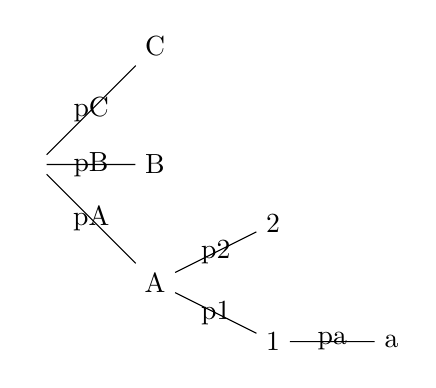
\begin{tikzpicture}[grow=right]

\node {}
child{node {A} child{node {1} 
						child{node {a} edge from parent node {pa}} 				edge from parent node {p1}} 
			   child{node {2} edge from parent node{p2} } 
edge from parent node{pA}}
child{node {B} edge from parent node{pB}}
child{node {C} edge from parent node{pC}}
;
\end{tikzpicture}


\end{document} 